% ---------------------------------------------------------------------------- %
%   PACKAGES AND OTHER LAYOUT CONFIGURATIONS                                   %
% ---------------------------------------------------------------------------- %
\documentclass[12pt,a4paper]{article}

% ---------------------------------------------------------------------------- %
%   a. Fonts, Language, Bibliography                                           %
% ---------------------------------------------------------------------------- %

\usepackage[utf8]{inputenc} % unicode characters
\usepackage[T1]{fontenc}    % Required for accented characters
\usepackage{ae,aecompl}     % Better Fonts
\usepackage{csquotes}       % recommended for babel
\usepackage{gensymb}        % Package for General Symbols (e.g. Celsius)
\usepackage{lscape}         % Landscape Mode
\usepackage{amsmath,amsfonts,amssymb,amsthm}
\usepackage{mathbbol}
\usepackage{accents}

% babel sillabation, british setup
\usepackage[british]{babel}%
% specify foreign words with
% \foreignlanguage{hlanguagei}{htexti}

% use natbib bibliography
\usepackage[semicolon,authoryear]{natbib}

% ---------------------------------------------------------------------------- %
%   b. Page Layout                                                             %
% ---------------------------------------------------------------------------- %

\marginparwidth   0pt
\oddsidemargin    0pt
\evensidemargin   0pt
\marginparsep     0pt
\topmargin      -40pt

\textwidth      6.5in
\textheight       9in

% Double spacing
% \renewcommand{\baselinestretch}{2}
% Do not indent
\setlength{\parindent}{0in}

% ---------------------------------------------------------------------------- %
%   c. General Utility Packages                                                %
% ---------------------------------------------------------------------------- %
\usepackage{alltt}     % to prevent memory overflow in case of long periods
\usepackage{lipsum}    % Used for inserting dummy 'Lorem ipsum' text
\newcounter{dummy}     % necessary for correct hyperlinks (to index, bib, etc.)
\newlength{\abcd}      % for ab..z string length calculation

% ---------------------------------------------------------------------------- %
%   d. Personal Data and User Ad-Hoc Commands                                  %
% ---------------------------------------------------------------------------- %
\newcommand{\HRule}{\rule{\linewidth}{0.5mm}} % Defines a new command for the horizontal lines, change thickness here

% for the footnote
\def\thanks#1{\footnote{#1}}
\renewcommand{\thefootnote}{\fnsymbol{footnote}}

% personal statements
\newcommand{\Title}{Does Culture Affect Households' Borrowing Choices?}%
\newcommand{\wDocument}{GSOEP Subsample Data Report}%
\newcommand{\Name}{Alessandro Pizzigolotto}%
\newcommand{\Supervisor}{Prof. Katrine V. Løken}%
\newcommand{\AffiliationA}{Norwegian School of Economics (NHH)}%
% \newcommand{\AffiliationB}{Università degli Studi di Padova}%
\newcommand{\Address}{Norges Handelshøyskole, Helleveien 30, 5045 Bergen, Norway}%
\newcommand{\Email}{\href{mailto:alessandro.pizzigolotto@nhh.no}{alessandro.pizzigolotto@nhh.no}}%

\usepackage[useregional]{datetime2} % to create new dates
% \newcommand{\mydate}{\DTMdisplaydate{2017}{02}{21}{-1}}
\newcommand{\mydate}{\today}

\makeatletter
\newcommand*\ExpandableInput[1]{\@@input#1 }
\makeatother


\newcommand*{\SummaryPath}{../../../res/summary}%

% ---------------------------------------------------------------------------- %
%   e. Floats, Figures, Tables, Code                                           %
% ---------------------------------------------------------------------------- %
\usepackage{graphicx} % Required for including pictures
\usepackage{wrapfig}  % Allows in-line images such as the example fish picture
\usepackage{subfig}   % allows to nest figures in the same environment creating panels
\usepackage{float}    % for using H in floats
\usepackage{caption}  % for caption setup
\usepackage{setspace}
\usepackage{enumerate}
\usepackage{booktabs}
\usepackage{multirow,array}
\captionsetup{justification=justified,%
    font={footnotesize,stretch=1,singlespacing}}
\captionsetup[subfloat]{position=top,textfont={it}, font={scriptsize}}

\usepackage[pdftex,hyperfootnotes=false,pdfpagelabels]{hyperref} % backref 
\pdfcompresslevel=9
\pdfadjustspacing=1
\hypersetup{%
    %draft, % = no hyperlinking at all (useful in b/w printouts)
    % colorlinks=true, linktocpage=true, pdfstartpage=3, pdfstartview=FitV,%
    % uncomment the following line if you want to have black links (e.g., for printing)
    colorlinks=false, linktocpage=false, pdfstartpage=1, pdfstartview=FitV,%
    pdfborder={0 0 0},%
    breaklinks=true, pdfpagemode=UseNone, pageanchor=true, pdfpagemode=UseOutlines,%
    plainpages=false, bookmarksnumbered, bookmarksopen=true, bookmarksopenlevel=1,%
    hypertexnames=true, pdfhighlight=/O,%nesting=true,%frenchlinks,%
    %urlcolor=webbrown, linkcolor=RoyalBlue, citecolor=webgreen, %pagecolor=RoyalBlue,%
    % urlcolor=Black, linkcolor=Black, citecolor=Black, %pagecolor=Black,%
    pdftitle={\Title},%
    % pdfauthor={\Name, \AffiliationA, \AffiliationB},%
    pdfauthor={\Name, \AffiliationA},%
    pdfsubject={Culture, Household Finance, Debt, Migration},%
    pdfkeywords={culture, migration, household finance, debt, microeconometrics},%
    pdfcreator={pdfLaTeX},%
    pdfproducer={\LaTeX with Sublime Text - Build 3211}%
}%

%----------------------------------------------------------------------------- %
%   BEGIN DOCUMENT                                                             %
%----------------------------------------------------------------------------- %

\begin{document}

%----------------------------------------------------------------------------- %
%   FRONTMATTER                                                                %
%----------------------------------------------------------------------------- %

\begin{center}
    {\Large \bf {\textup{\Title}}}\\
    \vspace{0.2in}
    {\large \sc \wDocument}\\
    \vspace{0.2in}
    {\bf {\Name}\thanks{\Name: \Address. \Email.}}\\
    % \AffiliationA, \AffiliationB\\
    \AffiliationA\\
    \vspace{0.3in}
    \mydate % Date
    \vspace{0.3in}
\end{center}

\section{Second-Generation Immigrants Identification}

In this document, I am briefly trying to shed some light on my work on the German Socio-Economic Panel (GSEOP) of the last period. \textit{In primis}, I start to describe my procedure, motivated by the technical report of \citet{bib:scheller2011}, with which I identify the (best possible number of) second-generation migrants in the SOEP longitudinal dataset. Suddenly, no code were available for this procedure or other components of this dataset. The method employs the following steps.

\begin{enumerate}
     \item In the tracking dataset, the generated variable \texttt{migback} allows me to identify whether individuals have an indirect, direct or no migration background, from which I select those individuals with an indirect migration background. From this group, I firstly retrieve their potential foreign nationality information from the variable \texttt{pgnation}: I prioritize this first variable to point out the country of ancestry, when available, amongst the next steps, and I save the information on an auxiliary variable to make the comparison with the next steps, where I will operate in the same fashion. To record this information, I coded a program that checks the frequency of the information within the targeted variables in the current and following steps. I calculate the mode of the information throughout the attainable waves and, when there is a multiple mode, I consider the most recent information available as the correct one. Within this approach, I also try to identify the specific country in case the country of ancestry is indicated as Ex-Yugoslavia for most of the waves.
     \item I proceed by merging the individual raw longitudinal dataset to firstly seek the information about citizenship and country of origin contained within the variables \texttt{pnat\_v1} and \texttt{pnat\_v2}, and the information about second nationality from the variable \texttt{pnat2}. Distinctly saving the information of those variables, I give to the former ones priority two and two the latter priority five when selecting the country of ancestry.
     \item Looking at the full longitudinal dataset, I consider the information from the variables \texttt{plj0018} and \texttt{plf0011} of previous nationality available in some waves, and the variable \texttt{plj0023} for second nationality in other waves. I save the former variables as the third source of information to identify the country of ancestry, whereas I merge the latter to the previous information on second nationality when it is missing.
     \item I check in the children's biographical dataset whether the respondent -- \textit{i.e.} the parent -- indicates the citizenship of those individuals, preferring this information to the second nationality from the previous data sources.
     \item I fetch across all the waves with a listed information about country of birth and previous nationalities -- from Wave A to Wave J -- to see whether they deviate from the previous information, or they integrate missing information at longitudinal level.
     \item I inspect the parents' biographical dataset, which contains information about parents' country of origin from the variables \texttt{forigin} and \texttt{morigin}. I consider maternal ancestry over paternal ancestry, and paternal ancestry where the mother is German-native or the maternal ancestry information is not available. When it is possible, I extract from the biographical dataset the parent identifier to link her survey information to the children, repeating all the previous steps valid for the children until I find a relevant information to characterize the country of ancestry.
     \item Respecting the priority stated within the previous steps, I save the country of ancestry information levelling up until the information is not missing. 
 \end{enumerate}

Figure~\ref{fig:bar_2ndgen_ancestry} illustrates the result of the previously described procedure. In the graph, I consider households where the household head is a second-generation migrant in working age, who is neither in education, nor retired. Furthermore, I exclude those households with missing information about outstanding loans/mortgages for the primary residence or other purposes.

\begin{figure}[htbp!]
    \centering
    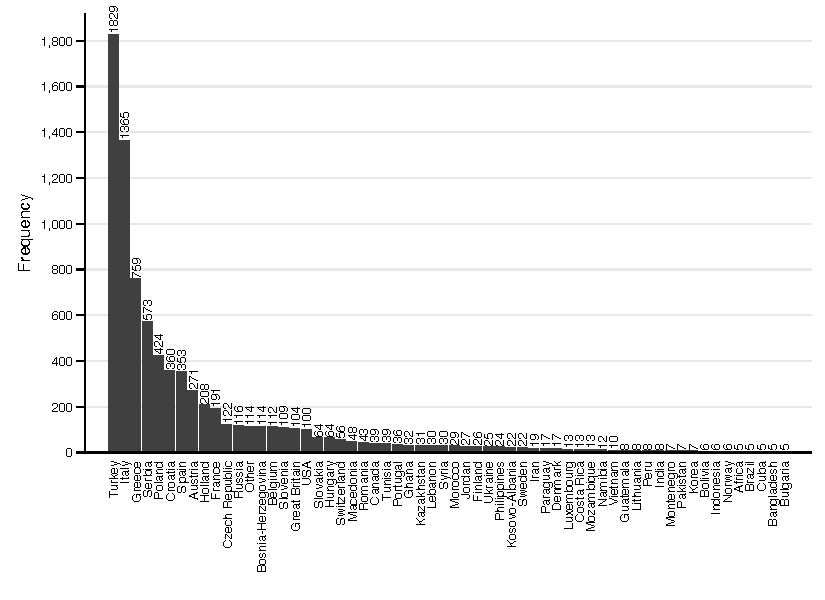
\includegraphics[width=\textwidth]{\SummaryPath/graphs/freq_total.pdf}
    \caption{Frequency of Second-Generation Household's Country of Ancestry (when identified). When the frequency is lower than $5$, country of ancestry is categorized as ``Other''. Individual Weighting Factor included. Years: $1984$-$2017$, households with missing information about loans are excluded. Source: German Socio-Economic Panel (GSOEP).}\label{fig:bar_2ndgen_ancestry}
\end{figure}

In Figure~\ref{fig:bar_2ndgen_year}, it is possible to observe how many households are disposable for each wave, conditional on the information about outstanding loans.

\section{Household Summary Statistics}

In the following tables, I summarize the main relevant variables I have been able to extract for the second-generation households. I will omit the full procedure I used to retrieve those variables, we can further discuss about this. In Table~\ref{tab:hhdemo}, it is possible to observe the head of household and the partner's demographics, weighted with the individual survey factors. Almost all variables cover the selected sample. Most all the variables are straightforward, except for the latest EGP value, which gives a measure of job prestige (the lower, the better job position), and the foreign identity scale (the higher, the less German identity) is constructed as the median value of five different questions in the individual longitudinal dataset harmonized throughout the waves: 

\begin{itemize}
    \item German feeling;
    \item connection with the country of origin;
    \item feeling of not belonging;
    \item feeling at home in the country of origin;
    \item wish to remain in Germany permanently.
\end{itemize}

Another peculiar variable is the usual language spoken by the individual in three levels, the higher the more fluent in the native language. Overall, the households are of young age, employed, and with vocational training.
In Table~\ref{tab:hhp_demo}, I describe the main relevant variables I am able to retrieve for the parents of the head of household and their current household, which are symmetrically summarized for the parents of the head of household's partner in Table~\ref{tab:hpp_demo}. Those variables are obtained both from the parents' biographical dataset and from the linking operation with the information of parents still in the survey. For the first-generation migrant parent, I am able to reconstruct the length of stay in Germany using the spell dataset of migration when available, the latest year of immigration, and the information about year of birth and death of the parent, which is also used for the current age. For some observations, we also have the information of closeness with the parent through the variable which measures the level of fights of the child with the parent at age 15.

In Table~\ref{tab:hh_info}, it is possible to observe the current household characteristics, and the main weakness of this dataset, other than the noticeable smaller sample size with respect to the original level of second-generation migrants in the longitudinal survey (roughly $13000$ amongst all the available waves, unconditional): information about household overall wealth is available just for three waves -- $2002$, $2007$ and $2012$ -- and most of the households are tenant, which I guess it is related to their young age. 

\begin{figure}[htbp!]
    \centering
    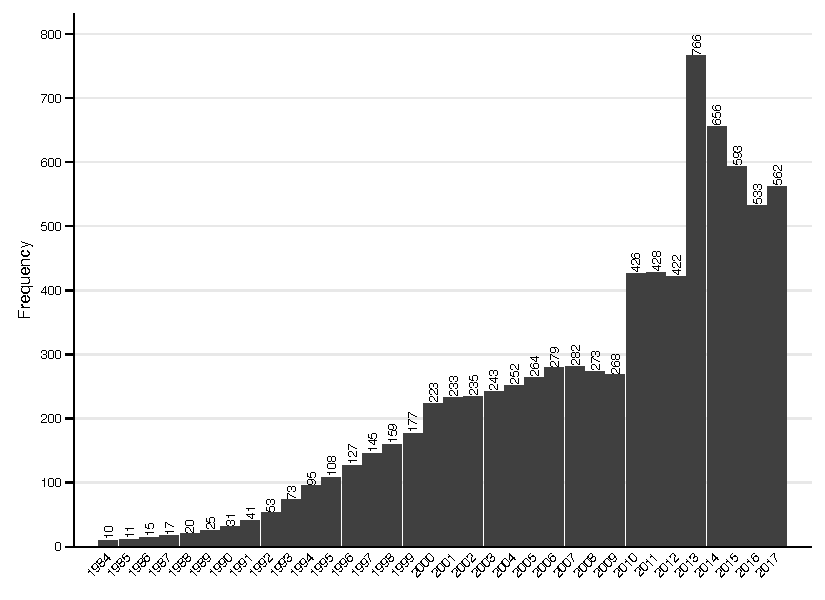
\includegraphics[width=\textwidth]{\SummaryPath/graphs/freq_years.pdf}
    \caption{Frequency of Second-Generation Household's Country of Ancestry by Year (when identified). Years: $1984$-$2017$, households with missing information about loans are excluded. Source: German Socio-Economic Panel (GSOEP).}\label{fig:bar_2ndgen_year}
\end{figure}

\begin{table}[htbp!]
    \centering
    \resizebox{\textwidth}{!}{%
        \begin{tabular}{l*{1}{ccccc}}
            \toprule
            \ & Mean & Std. Dev. & Min. & Max. & Obs.\\
            \midrule
            \multicolumn{6}{l}{\textbf{Panel A: Head of Household}}\\
            \midrule
            \ExpandableInput{\SummaryPath/tabs/summary_hh1}
            \midrule
            \multicolumn{6}{l}{\textbf{Panel B: Head of Household's Partner}}\\
            \midrule
            \ExpandableInput{\SummaryPath/tabs/summary_hh2}
            \bottomrule
        \end{tabular}
    }%
    \caption{Summary Statistics for Second-Generation Household Members' Demographics (with individual weighting factors). Years: $1984$-$2017$. Source: German Socio-Economic Panel (GSOEP).}\label{tab:hhdemo}
\end{table}

\begin{table}[htbp!]
    \centering
    \resizebox{\textwidth}{!}{%
        \begin{tabular}{l*{1}{ccccc}}
            \toprule
            \ & Mean & Std. Dev. & Min. & Max. & Obs.\\
            \midrule
            \multicolumn{6}{l}{\textbf{Panel A: Head of Household's Father}}\\
            \ExpandableInput{\SummaryPath/tabs/summary_hh4}
            \midrule
            \multicolumn{6}{l}{\textbf{Panel B: Head of Household's Mother}}\\
            \ExpandableInput{\SummaryPath/tabs/summary_hh5}
            \bottomrule
        \end{tabular}
    }%
    \caption{Summary Statistics for Second-Generation Head of Household's Parents (with head of household's weighting factor). Years: $1984$-$2017$. Source: German Socio-Economic Panel (GSOEP).}\label{tab:hhp_demo}
\end{table}

\begin{table}[htbp!]
    \centering
    \resizebox{\textwidth}{!}{%
        \begin{tabular}{l*{1}{ccccc}}
            \toprule
            \ & Mean & Std. Dev. & Min. & Max. & Obs.\\
            \midrule
            \multicolumn{6}{l}{\textbf{Panel A: Head of Household Partner's Father}}\\
            \ExpandableInput{\SummaryPath/tabs/summary_hh6}
            \midrule
            \multicolumn{6}{l}{\textbf{Panel B: Head of Household Partner's Mother}}\\
            \ExpandableInput{\SummaryPath/tabs/summary_hh7}
            \bottomrule
        \end{tabular}
    }%
    \caption{Summary Statistics for Second-Generation Head of Household Partner's Parents (with partner's weighting factor). Years: $1984$-$2017$. Source: German Socio-Economic Panel (GSOEP).}\label{tab:hpp_demo}
\end{table}



\begin{landscape}
\begin{table}[p]
    \centering
    \resizebox{\textheight}{!}{%
    \begin{tabular}{l*{1}{ccccc}}
        \toprule
        \ & Mean & Std. Dev. & Min. & Max. & Obs.\\
        \midrule
        \ExpandableInput{\SummaryPath/tabs/summary_hh3}
        \bottomrule
    \end{tabular}
    }\\%
    \parbox{\textheight}{\caption{Summary Statistics for the Current Second-Generation Household (with household weights). The Household Head is defined as the adult person, neither in education nor retired, who knows best about the general conditions under which the household acts and is supposed to answer this questionnaire in each given year. Years: $1984$-$2017$. Source: German Socio-Economic Panel (GSOEP).}\label{tab:hh_info}}
\end{table}
\end{landscape}

%----------------------------------------------------------------------------- %
%   REFERENCES                                                                 %
%----------------------------------------------------------------------------- %

% \printbibliography[title=\refname]
\bibliographystyle{agsm}
\bibliography{summary}

\end{document}